% F24 -- The life of one quiz question during a parse.
% Chapter 6 (Trusting the Machine). Drawn with TikZ at print width, included at scale 1.
% Claim supported: a generated question passes five stages before it is stored;
% three can drop it, the lexical score only flags it, a disputed key gets one
% repair pinned to the same page, and a failed check keeps the question.
% Sources: parser/synthesis.py:52 (cap 12), :63 (ENFORCE_SUPPORT_THRESHOLD = False),
% :75-80 (CHECK_ANSWERS, CHECK_MODEL), _map_deck_quiz; parser/quiz_grounding.py:25, :44;
% parser/quiz_validator.py (_normalize_answer_index); PR #166 (5ea0aeff); f25dd41c.
\documentclass[border=2pt]{standalone}
\usepackage[T1]{fontenc}
\usepackage{tgheros}
\renewcommand*\familydefault{\sfdefault}
\usepackage{tikz}
\usetikzlibrary{positioning,arrows.meta}
\begin{document}
\footnotesize
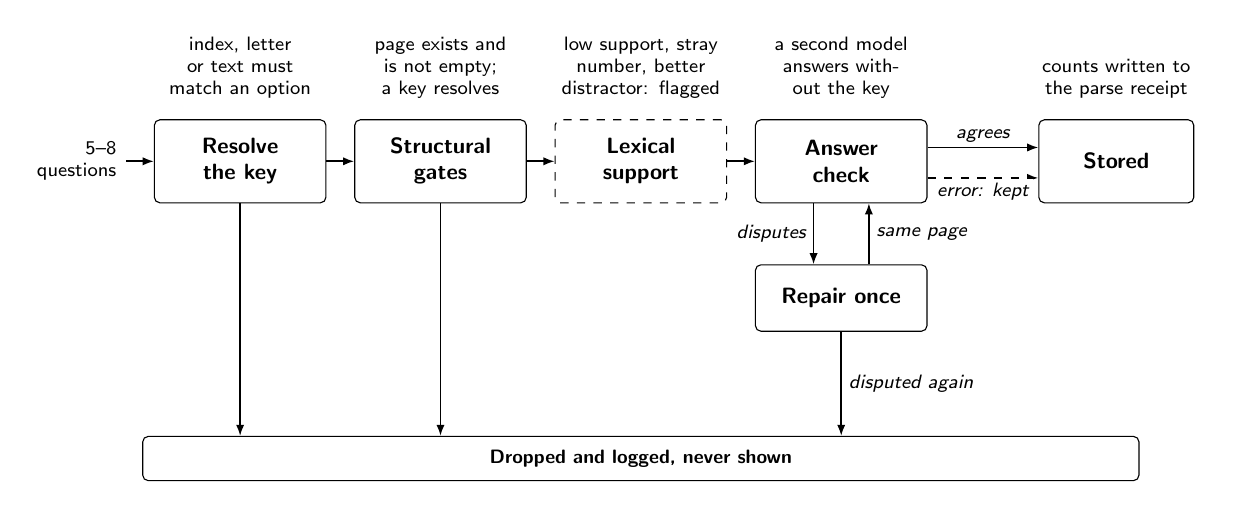
\begin{tikzpicture}[
  stage/.style={draw, rounded corners=2pt, minimum width=62pt, minimum height=30pt,
                align=center, inner sep=3pt, font=\footnotesize\bfseries},
  soft/.style={stage, dashed},
  note/.style={align=center, font=\scriptsize, text width=66pt},
  drop/.style={draw, rounded corners=2pt, minimum width=360pt, minimum height=16pt,
               align=center, font=\scriptsize\bfseries},
  lab/.style={font=\scriptsize\itshape, fill=white, inner sep=1.5pt},
  arr/.style={-{Latex[length=4pt]}, semithick},
  node distance=10pt]
  \node[stage] (key) {Resolve\\the key};
  \node[stage, right=of key] (str) {Structural\\gates};
  \node[soft,  right=of str] (lex) {Lexical\\support};
  \node[stage, right=of lex] (chk) {Answer\\check};
  \node[stage, right=40pt of chk, minimum width=56pt] (sto) {Stored};
  \node[font=\scriptsize, left=10pt of key, align=right] (gen) {5--8\\questions};
  \draw[arr] (gen) -- (key);
  \draw[arr] (key) -- (str); \draw[arr] (str) -- (lex);
  \draw[arr] (lex) -- (chk);
  \draw[arr] ([yshift=5pt]chk.east) -- node[lab, above=0pt] {agrees} ([yshift=5pt]sto.west);
  \node[note, above=4pt of key] {index, letter or text must match an option};
  \node[note, above=4pt of str] {page exists and is not empty; a key resolves};
  \node[note, above=4pt of lex] {low support, stray number, better distractor: flagged};
  \node[note, above=4pt of chk] {a second model answers without the key};
  \node[note, above=4pt of sto] {counts written to the parse receipt};
  \node[stage, below=22pt of chk, minimum height=24pt] (rep) {Repair once};
  \draw[arr] ([xshift=-10pt]chk.south) -- node[lab, left=1pt] {disputes} ([xshift=-10pt]rep.north);
  \draw[arr] ([xshift=10pt]rep.north) -- node[lab, right=1pt] {same page} ([xshift=10pt]chk.south);
  \node[drop, below=84pt of lex] (dr) {Dropped and logged, never shown};
  \draw[arr] (key.south) -- (key.south |- dr.north);
  \draw[arr] (str.south) -- (str.south |- dr.north);
  \draw[arr] (rep.south) -- node[lab, right=1pt] {disputed again} (rep.south |- dr.north);
  \draw[arr, dashed] ([yshift=-6pt]chk.east) -- node[lab, below=0pt] {error: kept} ([yshift=-6pt]sto.west);
\end{tikzpicture}
\end{document}
